\chapter{The Solution}
\label{ch:thesolution}

%
% Section: Scenario 
%
\section{Scenario}
\label{sec:thesolution:Scenario}

To manage the medical records of patients, need to map fabric components to requirements of the EHR systems. All hospitals act as organizations in fabric network. Patient data has been treated as assets which is stored in the ledger. It is also possible to store the reference of the EHR data in the ledger but since application is not managed by real data and for that it will be necessary to maintain the separate database which will have patients data. This can be a good solution when it is integrated with production or real hospitals EHR data. For now patient record has few fields like personal and medical details like age, address, allergies, symptoms, treatment, followup, etc. When doctor is medicating to a patient, patient history data will be available which helps doctors to assign appropriate treatment. To improve the privacy of records, it is designed to provide extra steps in application for patients. Patient can decide to have permission to access his/her data from a particular doctor. Doctor can view limited fields of assent means patient data like all medical fields along with age and allergies. Where as patient can view all the fields but edit only personal fields. 
A similar application approach also available in \cite{Dubovitskaya2020} which motivated to this solution further.

%
% Section: Why blockchain
%
\section{Why blockchain and fabric?}
\label{sec:thesolution:whyblockchain}

Blockchain has many advantages over many traditional database systems. One of the major advantages of blockchain is, it stores data cryptographically encrypted via distributed and decentralized way in peers which is nothing but a computing machine. This solves the availability of data within the network. It means for the outside world it is not possible to access data. The next benefit of blockchain is immutability. Since all the transactions are combined in a block and arranged in a chain as explained in Chapter \ref{ch:SOTA}. 

On top of the blockchain, hyperledger fabric provides some additional features which perfectly fit the current scenario. It is a permissioned and closed blockchain, no person can get added into the network unlike permissionless blockchains such as bitcoin, ethereum. This solves the confidentiality problem of patients' data. The fabric has a concept of Certificate Authority for every organization or common CA called Fabric CA and MSP which provides identities and verifies when a transaction request is made. Moreover, all the components of the fabric network are scalable and pluggable. It means more organizations can be added connected through channels, any number of peers for organizations. Like ethereum, the fabric also provides the concept of smart contracts, and when it is packaged and deployed it is called a chaincode. It is a business logic that is deployed on every endorsing peer. Initial organizations of the channel decide whether the new organizations should be added or not through Channel Configuration. It returns all the transaction information. All the components are explained further in the following section.

%
% Section: Use cases
%
\section{Use cases}
\label{sec:intro:Use cases}
There are three users in the system with role admin, patient, and doctor. Each user has its own use cases which are described in Figures \ref{fig:chapter03:admin use case}, \ref{fig:chapter03:patient use case} and \ref{fig:chapter03:doctor use case}. A user interfaces for admin from every hospital to make necessary changes about users.

\begin{figure}[htbp]
 \centering
 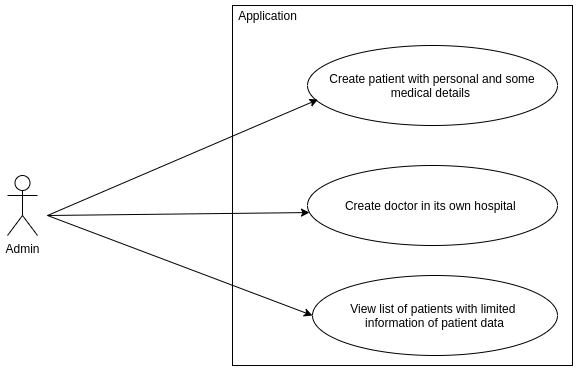
\includegraphics[width=1\textwidth, height=7cm]{gfx/figures/Admin use case .png}
 \caption{Admin use case diagram}
 \label{fig:chapter03:admin use case}
\end{figure}

\begin{figure}[htbp]
 \centering
 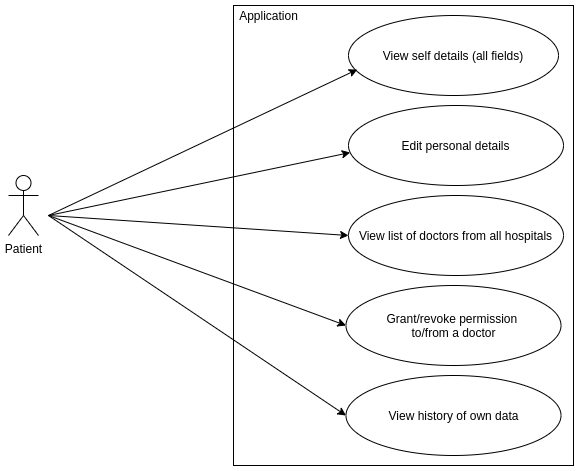
\includegraphics[width=1\textwidth, height=10cm]{gfx/figures/Patient use case.png}
 \caption{Patient Use case diagram}
 \label{fig:chapter03:patient use case}
\end{figure}

\begin{figure}[htbp]
 \centering
 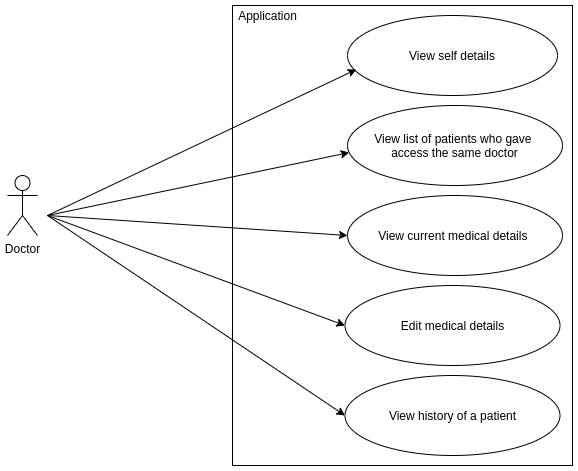
\includegraphics[width=1\textwidth, height=10cm]{gfx/figures/Doctor use case.png}
 \caption{Doctor Use case diagram}
 \label{fig:chapter03:doctor use case}
\end{figure}



%
% Section: Architecture
%
\section{Architecture}
\label{sec:implementation:architecture}

A high-level architecture of a system is depicted in Figure \ref{fig:chapter03:architecture}. The architecture also shows the fabric network in detail with color schemes. The blockchain operator setups the initial configuration of the network and provides necessary access and credentials to the users who govern the system. All the peers from the hospitals are nothing but docker containers of image hyperledger/fabric-peer, orderer, and ca. As described, every component of the application is pluggable, so backend code and smart contract are written in JavaScript language with ExpressJS as a server to provide REST API. The user interface is developed using the Angular 11 framework. The communication between the front and back end is performed through REST calls with JSON web token for authentication. Backend code can also be written in Java, Go, and Typescript which is officially supported languages by Hyperledger Fabric. For the given scenario single channel named 'hospitalChannel' and two hospital organizations are sufficient. The third hospital can also be successfully added in between when the network is running and gets joined with the same channel. 
Fabric provides support for two databases, LevelDB and CouchDB. The CouchDB is used for the solution because it is more flexible than LevelDB. Images handling is possible. It supports indexes, unlike LevelDB. Since all patient data stored in CouchDB and not maintaining any separate EHR store, CouchDB fits well. Whereas LevelDB is a powerful in-memory database developed by Google to store key-value pairs and in some cases, it is faster than CouchDB. The other use case scenario where the EHR database of hospitals is used and only stores references (maybe in the form of API) to that record in LevelDB as a blockchain ledger. Since use cases are simple here so CouchDB supports here properly. The ledger is a combination of the transaction log and world state. CouchDB is used to store the world state. Because of which no need to query the whole transaction log for every transaction request. Transaction log stores all transactions start from the first one which is stored in the genesis block. It can be found on local system at
\lstinline{/var/lib/docker/volumes/net\_peer0.org2.example.com/_data/ledgersData/chains/chains/mychannel/blockfile_000000} (depends upon the installation path). In Couchdb docker containers it is by default available at \lstinline{/var/hyperledger/production/ledgersData/chains/chains/mychannel/}. It is configurable in \href{https://github.com/kshitijyelpale/blockchain-hyperledger-fabric-electronic-patient-records/blob/main/app/first-network/docker/docker-compose-hospital-net.yaml}{docker-compose-hospital-net.yaml}. 
The Redis key-value DB is also used to store doctor credentials - username and password for doctor's credentials. Whereas other details of the doctor are stored as user attributes using fabric SDK.
The patient record has some personal and medical fields describe here in \href{https://github.com/kshitijyelpale/blockchain-hyperledger-fabric-electronic-patient-records/blob/main/app/patient-asset-transfer/chaincode/lib/initLedger.json}{initLedger} file. This is the initial data when the network gets up. Similarly, two doctors from every two hospitals are created.


\begin{figure}[htbp]
 \centering
 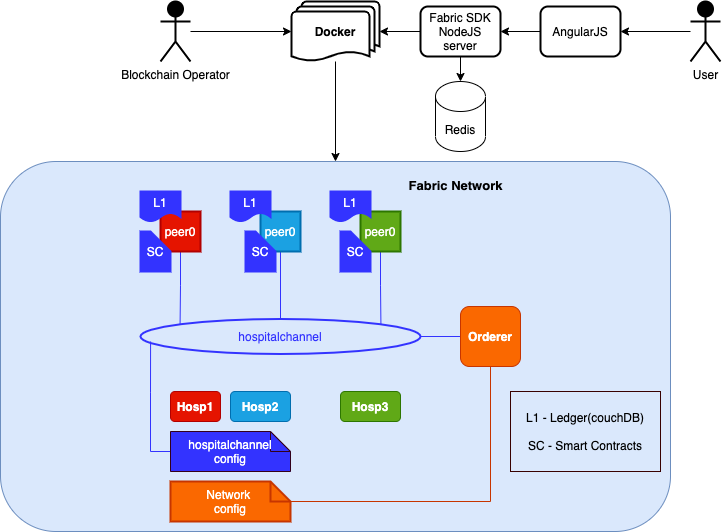
\includegraphics[width=1\textwidth, height=10cm]{gfx/figures/Architecture.png}
 \caption{Architecture}
 \label{fig:chapter03:architecture}
\end{figure}

% Section: Network/activity diagram
%
\section{Activity diagram}
\label{sec:thesolution:network/acitivitydiagram}

The Figure \ref{fig:chapter03:activityFirst} shows the interaction between components for creation of a patient. The patient needs to create an account only the first time the patient visits any one of the hospitals in the network, during the first visit the patient provides details to the admin, admin invokes the \lstinline{AdminContract} to create a patient. In the backend, firstly the admin certificate is used to connect to the network, and a transaction is created which adds the patient object to the ledger and also adds the patient identity to the blockchain network. After the creation of the patient is successful, the server creates a temporary password for the patient using which the patient can log in to the network. The patient credentials are added to the ledger as the patient can go to any of the hospitals in the network. The Figure \ref{fig:chapter03:activitySecond} shows the interaction to create a doctor. The doctor provides details to the admin, who then firstly connects to the network and then adds the doctor as an identity to the blockchain network. And the credentials of the doctor are stored in the hospital-specific Redis database. Now as patient and doctor are added as identities in the blockchain network, for the next interaction the patient/doctor can connect to the network using their certificates.

\begin{figure}[htbp]
 \centering
 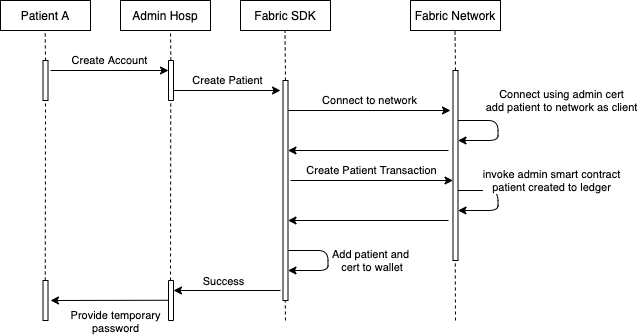
\includegraphics[height=6cm]{gfx/figures/first.png}
 \caption{Creation of a patient}
 \label{fig:chapter03:activityFirst}
\end{figure}

\begin{figure}[htbp]
 \centering
 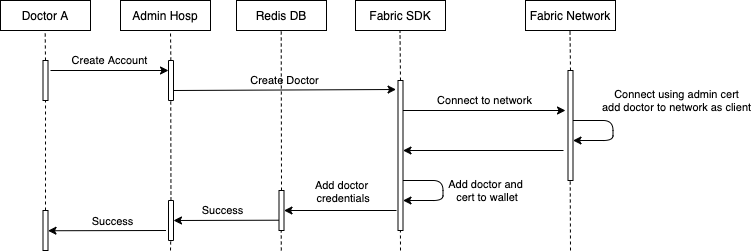
\includegraphics[height=5cm]{gfx/figures/second.png}
 \caption{Creation of a doctor}
 \label{fig:chapter03:activitySecond}
\end{figure}


\section{Applying Fabric Components}
\label{sec:thesolution:fabriccomponents}
The HLF comprises many components, has a complex architecture. And these components can be applied and used in many various ways. The following describes how HLF components are applied.

\subsection{Smart Contract \& Chaincode}
A smart contract in hyperledger fabric defines the transaction logic that controls the lifecycle of a business object contained in the world state \cite{Smart-Contracts-Chaincode}. Mutiple Smart contracts are packaged into a single chaincode which is then deployed to a blockchain network. A smart contract defines the rules between different organizations in executable code. Fabric SDK invokes a smart contract to create transactions which then performs changes to the ledger. A smart contract is defined within a chaincode. Multiple smart contracts can be defined within the same chaincode. When a chaincode is deployed, all smart contracts within it are made available to applications.
As shown in Figure \ref{fig:chapter03:smartContractHierarchy} the application comprises mainly three smart contracts packaged into a single chaincode - each role (Patient/Doctor/Admin) invokes its very own smart contract.
\begin{itemize}
    \item \lstinline{AdminContract} - This contract is invoked by the admin. The methods in the contract give the admin the ability to create/delete patients by adding/deleting patient object to from the ledger. Admin can also view all the patients available throughout the network. 
    \item \lstinline{PatientContract} - The patient interacts with the ledger by invoking this contract. The contract contains the logic that is required for the patient. For instance, only the patient can update/view the personal details and password via the methods defined in the contract. And also patient contract contains methods to grant and revoke access to from a doctor. 
    \item \lstinline{DoctorContract} - The doctor contract has methods that allows the doctor to update/read the patients medical details. 
\end{itemize}
The idealogy for the three smart contracts is to make sure that the right role has the right access to the data on the ledger. Only the patient has the right to update the personal details, grant/revoke access, and update the password. These methods can be invoked by neither the admin nor the doctor. And similarly, the methods of the doctor cannot be accessed by the patient or admin. The read patient method is common for all, but the data which is retrieved by the contract is different for each role admin just has the access to patient name, the doctor has the access to the medical details and the patient has the access to the whole object. 

\begin{figure}[htbp]
 \centering
 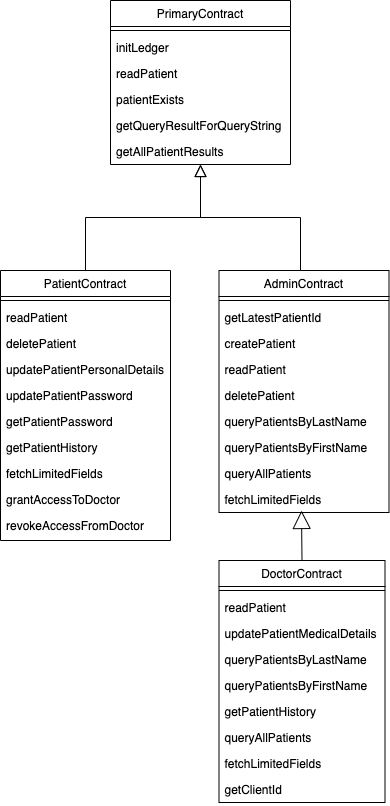
\includegraphics[width=6cm, height=10cm]{gfx/figures/smartContractHierarchy.png}
 \caption{Smart Contracts Hierarchy}
 \label{fig:chapter03:smartContractHierarchy}
\end{figure}

\subsection{Endorsement policies}
The chaincodes in Hyperledger fabric have an endorsement policy that specifies the peers on the channel that executes the chaincode functions and endorses the results to the ledger and makes the transaction valid. The endorsement policies define the peers which will verify and approve/reject the execution of a transaction. During this process, the peers verify the transaction, and the committing peer ensures sure that the transaction contains the the required number of endorsements which is configured in the endorsement policy.\cite{Policies}.

The Endorsement Policy is defined in the \href{https://github.com/kshitijyelpale/blockchain-hyperledger-fabric-electronic-patient-records/blob/main/app/first-network/configtx/configtx.yaml}{configtx.yaml}. Each hospital contains its very own endorsing peers as specified in the YAML file in the path \lstinline{&hosp1/Policies/Endorsement} similarly for hosp2. The rule specifies the roles who are endorsers. In the YAML file, all the peers of the hospitals are endorsers. A Chaincode-level endorsement policy is defined in the YAML file in the PATH Application: \lstinline{&ApplicationDefaults/Policies/Endorsement} \lstinline{`MAJORITY`} specifies that only when a majority of channel members approve a chaincode definition then definition iscommitted to the channel.

\subsection{Endorsing members of hospitals}
In path \lstinline{&hosp1/Policies/Endorsement} the rule \lstinline{OR('hosp1MSP.peer')}  requests one signature from the peers of hosp1. Other values can be : \\ 
\begin{itemize}
    \item Requests one signature from each role 
        \begin{lstlisting}
            AND('hosp1MSP.peer', 'hosp1MSP.admin')
        \end{lstlisting} 
    \item Requests one signature from either one of the roles 
        \begin{lstlisting}
            OR('hosp1MSP.peer', 'hosp1MSP.admin') 
        \end{lstlisting} 
\end{itemize}

\subsection{Specifying the endorsing policy}
In path \lstinline{&ApplicationDefaults/Policies/Endorsement} other types can be a signature with the one of the following rules:
\begin{itemize}
    \item A transaction is commited only if admin of the both the hospital approve.
        \begin{lstlisting}
            AND('hosp1MSP.admin', 'hosp2MSP.admin') 
        \end{lstlisting} 
    \item A transaction is commited only if either one of the admin of the both the hospital approve. 
        \begin{lstlisting}
            OR('hosp1MSP.admin', 'hosp2MSP.admin')
        \end{lstlisting} 
    \item \lstinline{OutOf(1, 'hosp1MSP.admin', 'hosp2MSP.admin')} which is equivalent to \lstinline{OR('hosp1MSP.admin', 'hosp2MSP.admin')}
\end{itemize}

\subsection{Ledger}
A Distributed ledger in Hyperledger Fabric as shown in Figure \ref{fig:chapter03:ledger} - one that is logically singular, but has many consistent copies distributed throughout a network comprises of two parts - the world state which holds the current values of the objects, the other part is the blockchain which is the history of the transactions which resulted to the current world state\cite{Ledger}.

\begin{figure}[htbp]
 \centering
 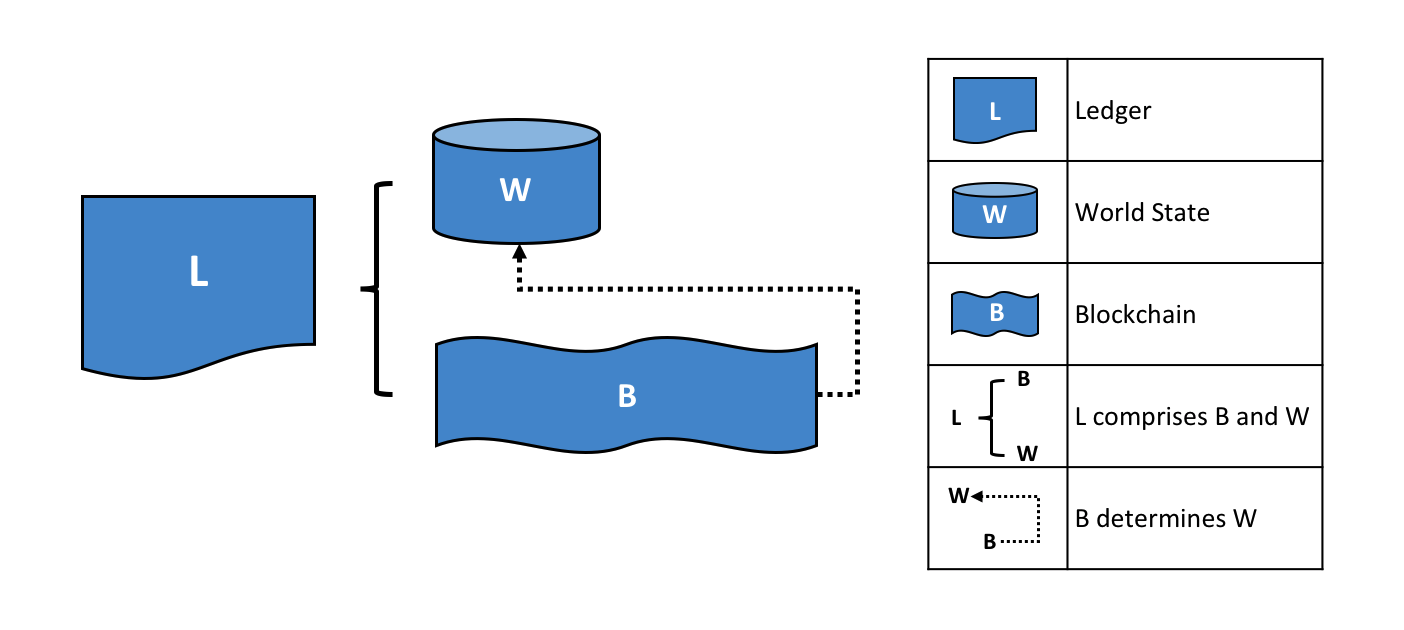
\includegraphics[width=10cm, height=6cm]{gfx/figures/ledger.diagram.1.png}
 \caption{Ledger in Hyperledger Fabric \cite{Ledger}}
 \label{fig:chapter03:ledger}
\end{figure}

In the application, the idealogy of a ledger can be thought of as one logical database in a Hyperledger Fabric network. In reality, the network contains multiple copies of a ledger for each hospital's peers – which are kept consistent with every other copy through consensus. The ledger in the application is being utilized in the following ways 
\begin{itemize}
    \item Firstly, the world state is the database where all the patient data is stored. All patients that are queried and updated are stored in the world state. All the query transactions are retrieved from the world state.
    \item Secondly, the transaction log which is a sequential structured interlinked blocks of log files, where each block contains a sequence of transactions, and a transaction represents a query or an update to the world state. The getHistory API specifically  uses the  transaction log to retrieve the history of an asset.
\end{itemize}

\subsection{Identity (CA)}
For a participant of a hospital, the participants first need to prove that can be are trusted to make transactions in the blockchain network. An identity for each participant issued by a trusted authority is required to be recognized in this network \cite{Identity}. The MSPs are the trusted authorities - which can be found in \href{https://github.com/kshitijyelpale/blockchain-hyperledger-fabric-electronic-patient-records/blob/main/app/first-network/configtx/configtx.yaml}{configtx.yaml}. An Hospital Certificate Authority(CA) dispenses certificates to each of its participants. These certificates are digitally signed by the CA and bind together the participant with the participant’s public key with a set of permissions. As a result, if one trusts the CA (and knows its public key), it can trust that the specific participant bound to the public key included in the certificate by validating the CA’s signature on the participant’s certificate. In the application either CAs(default) or cryptogen can be used to issue identities in the network: 
\begin{itemize}
    \item \emph{Cryptogen}: Cryptogen is a tool that creates certificates and keys. This tool can be used during development and testing. The tool quickly just creates the required crypto material for the hospitals\cite{Cryptogen}. The configuration files for all the hospitals and the orderer are defined in \href{https://github.com/kshitijyelpale/blockchain-hyperledger-fabric-electronic-patient-records/tree/main/app/first-network/organizations/cryptogen}{cryptogen} directory, the \lstinline{YAML} files contain the necessary information for the tool to create the cryto material for the hospitals and the Orderer.
    \item \emph{CAs}: Each hospital has its very own CA server that creates the identities using client of the server to prove that the identity belong to their hospital and can be trsuted. All of the identities created by a CA run of the hospital share the same trust of the root CA \cite{Identity}. The application uses CAs to allows registration and enrolling patients/doctors with the Fabric SDK which cannot be done using Cryptogen. The configuration files of the CAs of the hospitals and orderer defined in \href{https://github.com/kshitijyelpale/blockchain-hyperledger-fabric-electronic-patient-records/blob/main/app/first-network/organizations/fabric-ca/hosp1/fabric-ca-server-config.yaml}{Hosp1CA}, \href{https://github.com/kshitijyelpale/blockchain-hyperledger-fabric-electronic-patient-records/blob/main/app/first-network/organizations/fabric-ca/hosp2/fabric-ca-server-config.yaml}{Hosp2CA} and \href{https://github.com/kshitijyelpale/blockchain-hyperledger-fabric-electronic-patient-records/blob/main/app/first-network/organizations/fabric-ca/ordererOrg/fabric-ca-server-config.yaml}{OrdererCA} respectively. 
\end{itemize}


\subsection{Membership Service Provider (MSP)}
Hyperledger Fabric is a permissioned blockchain network, all the participants of the network, in our application the peers/doctors/patients need to prove their identity to join and perform transactions in the blockchain network to prove that these participants can be trusted. Hyperledger Fabric uses a Public Key Infrastructure (PKI) \cite{MSP} to verify identities in a chain of trust. The fabric uses Certificate Authorities(CA) to prove identity, the CAs generate a public and a private key for each identity which forms a key-pair using which the participants can prove their identity and be recognized in the network. The MSP is the one that verifies the private keys of the participants by matching them with the stored public key. For instance, in the application the peers of the hospital endorse a transaction using its private key, the MSP on the ordering service is where the public key is stored which is used to verify that the private key attached to the transaction is valid. CAs are used to create trusted identities that are recognized by the network(peers/doctors/patients). MSPs are used for defining the hospitals that are trusted by the network members. MSPs are allocated the participants of the hospitals with a set of roles and permissions within the network. In the applications, all the hospitals that join the network can perform read/write transactions in the network. These permissions are configured in \href{https://github.com/kshitijyelpale/blockchain-hyperledger-fabric-electronic-patient-records/blob/main/app/first-network/configtx/configtx.yaml}{configtx.yaml} and for participants of these hospitals to perform a transaction in the network they first have to have an identity issued by a CA that is recognized in the network. And be a member of any of the hospitals - MSP is how the participants are linked as a member to the hospital, this is when the public key of the participant is stored in the hospital MSP.

%
% Section: Security Mechanisms
%
\section{Security Mechanisms}
\label{sec:thesolution:securitymechanisms}
Security of the data is essential when question arises for patient data in medical data. Blockchain concept is very safe and secure itself and provides a mechanism of chaining in which if any transaction changes all successive blocks needs to change which is a very heavy task. In addition to that in hyperledger fabric when new peer and or organizations joins the channel approved by in channel configuration, still it should not be exposed, as it is available for all kind of peers. To avoid that data can be encrypted or hidden based on patient's grant/revoke actions for doctors. The proof of concepts of two mechanisms are described further. Unfortunately it is not yet implemented due to some unavoidable reasons. 

\subsection{Private Collections}
The data used and stored in Healthcare is highly confidential and must be secure. The data of the patient must be private to only the hospitals or doctors that the patient has allowed access to. Hyperledger Fabric contains functionality to store private data using private data collections\cite{Privatedata}. Private data is the data that must be kept private from other hospitals or doctors. A private data collection contains two elements:
\begin{itemize}
    \item \emph{The actual private data}: Only the data of the private collections that are authorized for particular hospitals can be accessed. 
    \item \emph{A hash of that data}: Patient data for which the hospital does not have the authorization, this data is hashed and stored and cannot be accessed by the member of the hospital.
\end{itemize}
In this application, there are n! + 1 number of private data collections where n is the number of hospitals. For instance, if there are 3 hospitals, there will be 7 private data collections. There will be a private data collection for each combination such as there will be a private collection for each hospital and a private collection which will be shared by any two hospitals and one private data collection shared by all the hospitals. The patient data stored on the collection depends on the doctors to which patient has authorized. If the patient has authorized to only one hospital, this will be stored in the private collection of that hospital. Now if the patient grants access to a doctor of another hospital, the private data is moved from the current collections to the collection which is private to the two hospitals. There will be no duplicate of the data. The patient data will always be in any one of the private data collection. The same mechanisms are applied when the patient revokes access from a hospital.

\subsubsection{Implementation Example}

Let us consider if there are two hospitals named Hospital 1 and Hospital 2. There will be a total of 3 private data collections named \lstinline{Hosp1PrivateCollection} which contains patient data which is authorized only for Hospital 1 similar \lstinline{Hosp2PrivateCollection} and a collection named \lstinline{Hosp12PrivateCollection} which is private to both Hospital 1 and Hospital 2, in this collection the patient would have granted access to both the hospitals. The channel world state will contain the assedId and the collection in which the asset is stored. This makes the reading of the patient data faster. 

\subsubsection{Scenarios}
\begin{itemize}
    \item \emph{Read/Update Patient}: First the patientId is read on the world state which will give the private data collection name, and then the patient data is read/updated from that private collecion.
    \item \emph{Grant/Revoke access to a new Hospital}: For instance if a patient is present in \lstinline{Hosp1PrivateCollection} and this patient grants access to Hospital 2, The data is first copied into \lstinline{Hosp12PrivateCollection} and then deleted in \lstinline{Hosp1PrivateCollection}.
    \item \emph{Get History}: The private data collections has not been implemented yet in the application due to the work in progress.Read the section for more details in Chapter \ref{sec:results:issues:getHistoryForKey}
\end{itemize}

\begin{figure}[htbp]
 \centering
 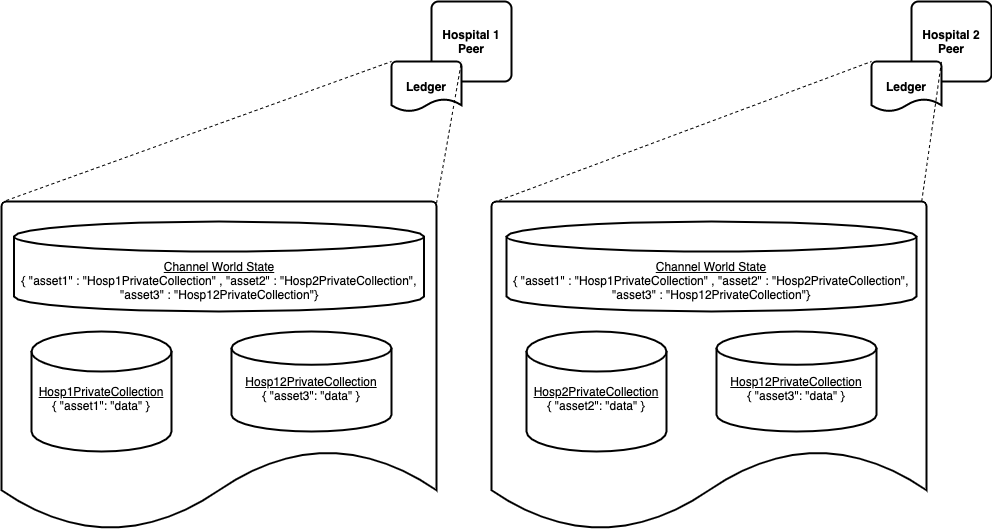
\includegraphics[width=1\textwidth, height=6cm]{gfx/figures/PrivateChannel.png}
 \caption{Private Data Collections}
 \label{fig:chapter03:privateCollection}
\end{figure}

\subsection{Data re-encryption}

It is a very common technique to store data in an encrypted format and decrypt it whenever is required. There are two types of encryption - Symmetric and asymmetric encryption. In the symmetric encryption technique, a common key is used to encrypt and decrypt the data. Whereas two different keys are used in asymmetric cryptographic encryption methods which are called private and public keys. It is also called public-key cryptography. RSA (Rivest–Shamir–Adleman) is a common algorithm used by modern computers to encrypt and decrypt data. 
typical use case, user A sends data to user B by encrypting data using user B's public key. Public keys are publically available for usage. To prove the authenticity of a public key, it is signed by some authority using a digital signature. Certificate Authority is an entity that issues a digital certificate. A digital certificate certifies the ownership of a public key of a user or an organization. So when user B receives data, it is decrypted by its private key. In the reverse mechanism, i.e., data encrypted by a private key and decrypted by the public key used in case of authentication a user.


\begin{figure}[htbp]
 \centering
 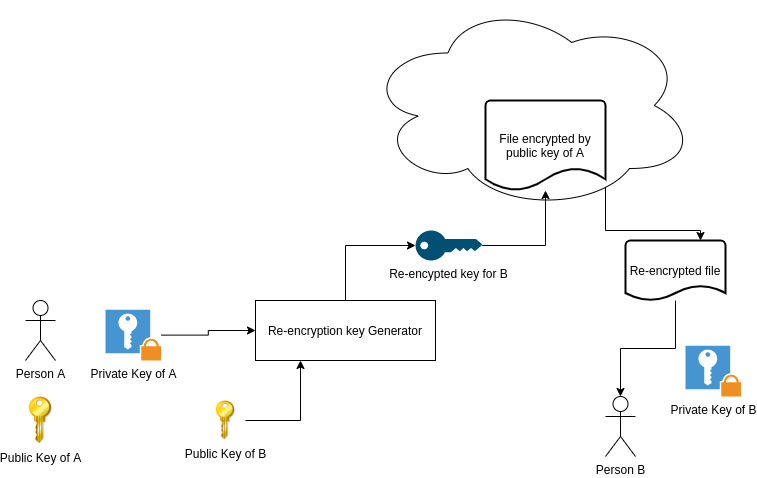
\includegraphics[width=1\textwidth, height=8cm]{gfx/figures/Re-encryption.png}
 \caption{Re-encryption}
 \label{fig:chapter03:reencryption}
\end{figure}

Consider the scenario depicted in Figure \ref{fig:chapter03:reencryption}. Person A has a data file on the cloud and person B wants to access the data. So typically, person A has to download the file, encrypt it with person B's public key, and then person B can decrypt it with its private key. These steps have some limitations. Person A needs to download the file and do encryption which is not feasible as the file size can be large and after encryption person needs to upload. So in the re-encryption approach, person A generates a re-encryption key from its private key and person B's public key, so it is a combination. This key sends to person B and the person re-encrypts the cloud file. The file is already encrypted by person A's public key but it encrypts again with the re-encryption key so the name is that way. After re-encryption, person B decrypts the file using its private key \cite{Tith2020}. Now even if the re-encryption key is lost or someones else found it, still at the end it needs to be decrypted by person B's private key. So it is secure.
The same approach can be applied in this scenario. The patient record would look as follows:

\begin{lstlisting}[language=json,firstnumber=1]
{
"patientId": "p1",
"password": hash(pwd),
"pwdTemp": true
"firstName": "abc",
"lastName" "xyz",
"data": encrypted patient data using symmetric key,
"changedBy": "doctorId XX",
"permissionGranted": [doctorId1: re-encrypted key for doctor 1, doctorId2: re-encrypted key for doctor 2, ...],
"encryptedSymmetricKey" : "######"
}    
\end{lstlisting}

All personal and medical fields are encrypted by some randomly generated key which is used as a symmetric key and stored in data as shown above. The symmetric key is also encrypted by the patient's public key and stored in the ledger under 'encryptedSymmetricKey' field. The reason behind using both encryption methods is, that a symmetric key is mostly recommended to encrypt large data. So when a patient provides access to a doctor then the re-encrypted key is calculated and stored with doctorId in the 'permissionGranted' field. So that when the doctor reads the ledger, if that doctorId is present then that re-encrypted key can be used to re-encrypt the 'encryptedSymmetricKey' and then decrypt using the doctor's private key. Once a doctor gets a symmetric key then it can easily be used to decrypt data. So basically data is encrypted only by symmetric but a re-encryption mechanism is applied to hide the symmetric key so it makes the mechanism quite robust. 

